%!TEX root = ../report.tex

\begin{document}
    \chapter{Results and Evaluation}

    The results of experiments conducted in this work as described in the \autoref{chap:experiment_setup} have been discussed here. The performance of models and different active learning query strategies have been studied using metrics such as accuracy, F1 score, kappa score and average time taken for each query. In addition, we analyze the performance of the query strategy-model combinations using a bump plot (which shows the ranking of each combination with respect to the accuracy as the number of queries increases). This unique plot enables to track the performance of any combination and helps in determining the consistent strategies and the models associated with them. Bump chart gives a more clear insight when compared to the accuracy plots which are intertwined in most of the cases.
    
    In order to observe the efficiency of active learning, every model-query strategy combination is compared with passive learning where the query instances are sampled randomly. For every dataset, we select the best active learning setting and compare the results with that of supervised learning. Here, the supervised learning models were trained with a dataset (which was obtained by a random split) of size comparable to that of active learning setting. The plot for supervised learning was obtained by averaging the results after 10 iterations. 
    
    The graphs depict the performance of different settings with respect to the number of queries made to the human grader in order to get his/her grades. The models were trained from the queried answers and the performances were calculated based on the grades assigned to the remaining answers. For e.g., if 10\% of the data were queried from a human, the remaining 90\% of the data was used to calculate the performance. From the model's performances based on the features used, accuracy and F1 scores, the best ones were selected to be viewed as a bump chart.
    
    \section{Experiment 1: Mohler'11 Dataset using Features from Sultan'16}
	
	This experiment was done using Sultan'16 features which were obtained as shown in Fig \ref{sultan_features}. The task of grading was split into binary classification and multi-class classification. The objective of binary classification is to identify correct and incorrect answers whereas multi-class classification's objective is to assign the correct grade for each answer. 
	
	\subsection{Binary Classification}
	
	The experimental results of different model-query strategy combinations in a binary classification setting are shown in Fig \ref{t1_b_uncertainty} and \ref{t1_b_com}. As the class distribution of this dataset is uneven, accuracy alone would not be enough to judge the performance of the models. Hence, the results were also analyzed using the F1 score which are shown in Fig \ref{t1_b_uncertainty_f1} and Fig \ref{t1_b_com_f1}.
	
	\begin{figure}[!htb]
		\centering
		\includegraphics[scale=0.46]{images/binary/task1_accuracy_uncertainty}
		\caption{Results in terms of accuracy for different models with uncertainty based query strategies.}
		\label{t1_b_uncertainty}
	\end{figure}
	
	\begin{figure}[!htb]
		\centering
		\includegraphics[scale=0.46]{images/binary/task1_f1score_uncertainty}
		\caption{Results in terms of F1 score for different models with uncertainty based query strategies.}
		\label{t1_b_uncertainty_f1}
	\end{figure}
	
	
	\begin{figure}[!htb]
		\begin{subfigure}[b]{0.5\textwidth}
			\includegraphics[width=\textwidth]{images/binary/task1_accuracy_com}
			\caption{Results in terms of accuracy for committee based query strategies.}
			\label{t1_b_com}
		\end{subfigure}
		~
		\begin{subfigure}[b]{0.5\textwidth}
			\includegraphics[width=\textwidth]{images/binary/task1_f1score_com}
			\caption{Results in terms of F1 score for committee based query strategies.}
			\label{t1_b_com_f1}
		\end{subfigure}
		~
		\caption{Committee-based binary classification.}
	\end{figure}
	
	Based on these graphs, we observe that all the active learning query strategies outperform the passive learning. We also observe that all the active learning strategies in their respective models performed comparably to each other. Hence, we selected the margin based uncertainty sampling for each model in order to compare them using a bump chart. This chart shows the performance of every model ranked by their accuracies which is shown in Fig \ref{t1_b_bump}. The bump chart for binary classification shows that all the models compete each other for the best performance and it is impossible to chose a clear consistent winner out of these. 
	
	\begin{figure}[!htb]
		\centering
		\includegraphics[scale=0.3]{images/binary/task1_rank}
		\caption{Bump chart of model performance in binary classification.}
		\label{t1_b_bump}
	\end{figure}
	
	
	
%	Fig \ref{t1_b_best} shows the comparison between the performance of the best model in active learning setting and in a supervised learning setting with random splits.
%	
%	\begin{figure}[!htb]
%		\centering
%		\includegraphics[scale=0.35]{images/binary/task1_best}
%		\caption{Active vs. supervised learning for binary classification with Sultan'16 features.}
%		\label{t1_b_best}
%	\end{figure}
	
	
	
	%================================================
	\clearpage
	\subsection{Multi-class Classification}

	The experimental results of different model-query strategy combinations in a multi-class classification setting are shown in Fig \ref{t1_m_uncertainty} and \ref{t1_m_com}. The results were also analyzed using the F1 score which are shown in Fig \ref{t1_m_uncertainty_f1} and Fig \ref{t1_m_com_f1}.
	
	\begin{figure}[!htb]
		\centering
		\includegraphics[scale=0.45]{images/task1_accuracy_uncertainty}
		\caption{Results in terms of accuracy for different models with uncertainty based query strategies.}
		\label{t1_m_uncertainty}
	\end{figure}
	
	\begin{figure}[!htb]
		\centering
		\includegraphics[scale=0.45]{images/task1_f1score_uncertainty}
		\caption{Results in terms of F1 score for different models with uncertainty based query strategies.}
		\label{t1_m_uncertainty_f1}
	\end{figure}
	
	
	\begin{figure}[!htb]
		\begin{subfigure}[b]{0.5\textwidth}
			\includegraphics[width=\textwidth]{images/task1_accuracy_com}
			\caption{Results in terms of accuracy for committee based query strategies.}
			\label{t1_m_com}
		\end{subfigure}
		~
		\begin{subfigure}[b]{0.5\textwidth}
			\includegraphics[width=\textwidth]{images/task1_f1score_com}
			\caption{Results in terms of F1 score for committee based query strategies.}
			\label{t1_m_com_f1}
		\end{subfigure}
		~
		\caption{Committee-based multi-class classification.}
	\end{figure}
	
	We observe that all the active learning query strategies outperform the passive learning (random sampling). Considering the accuracy and the F1 scores, logistic regression with margin uncertainty sampling, naive Bayes with margin uncertainty sampling, random forest with uncertainty sampling, and linear SVM with margin uncertainty sampling were selected for comparison using a bump chart. In case of committee, max disagreement sampling performed better and is added to the bump chart comparison. This chart shows the performance of every model ranked by their accuracies which is shown in Fig \ref{t1_m_bump}.
	
	\begin{figure}[h]
		\centering
		\includegraphics[scale=0.3]{images/task1_rank}
		\caption{Bump chart of model performance in multi-class classification.}
		\label{t1_m_bump}
	\end{figure}
	
	The bump chart clearly shows that the random forest classifier model with least confident uncertainty sampling is preferable over logistic regression for this setting. Random forest classifier shows consistent performance over the whole range of queries. 
	
	The time comparison of different models is tabulated in Table \ref{task1_m_time}. Based on the bump plot and time comparison, it could be inferred that random forest with least confident uncertainty sampling is best for Mohler'11 dataset with Sultan'16 features.  
	
	\begin{table}[!htb]
		\centering
		\scalebox{0.6}{
			\begin{tabular}{|c|c|c|c|c|c|c|}
				\hline
				& \multicolumn{6}{c|}{\textbf{Time taken per query (secs)}} \\ \hline
				\textbf{Models} & \textbf{\begin{tabular}[c]{@{}c@{}}least confident\\ uncertainty\end{tabular}} & \textbf{\begin{tabular}[c]{@{}c@{}}margin based \\ uncertainty\end{tabular}} & \textbf{\begin{tabular}[c]{@{}c@{}}entropy based \\ uncertainty\end{tabular}} & \textbf{\begin{tabular}[c]{@{}c@{}}vote \\ entropy\end{tabular}} & \textbf{\begin{tabular}[c]{@{}c@{}}max\\ disagreement\end{tabular}} & \textbf{\begin{tabular}[c]{@{}c@{}}consensus \\ entropy\end{tabular}} \\ \hline
				Logistic Regression & 0.0145 & 0.0150 & 0.0151 & \multirow{3}{*}{0.4220} & \multirow{3}{*}{0.4211} & \multirow{3}{*}{0.4184} \\ \cline{1-4}
				Naive Bayes & 0.0059 & 0.0062 & 0.0064 &  &  &  \\ \cline{1-4}
				\begin{tabular}[c]{@{}c@{}}Random Forest \\ (100 trees)\end{tabular} & 0.3216 & 0.3235 & 0.3182 &  &  &  \\ \hline
				SVC - Linear & 0.1341 & 0.1305 & 0.1354 & - & - & - \\ \hline
				SVC - RBF & 0.3869 & 0.3843 & 0.3879 & - & - & - \\ \hline
			\end{tabular}}
			\caption{Time comparison between different models for multi-class classification.}
			\label{task1_m_time}
		\end{table}
	
%	Fig \ref{t1_m_best} shows the comparison between the performance of the best model in active learning setting and in a supervised learning setting with random splits.
%	
%	\begin{figure}[h]
%		\centering
%		\includegraphics[scale=0.35]{images/task1_best}
%		\caption{Active vs. supervised learning for multi-class classification with Sultan'16 features.}
%		\label{t1_m_best}
%	\end{figure}

	\clearpage
	
 \section{Experiment 2: Mohler'11 Dataset using Bag-of-words (BOW) Features}
 
 Instead of Sultan'16 features, Bag-of-words(BOW) of the answers were used as features for this experiment. Extracting this feature doesn't require reference answers of the questions as the entire BOW vectors were created from the student answers alone. Every answer was encoded into a vector of length 2138 and this vector was used as input to our models during training and prediction. The linear SVC and RBF kernel SVC models were ignored in this experiment as they consume a lot of time to select each query since the dimension of the feature space is very high. Considering the future implementation of this project as an interactive task, time becomes a key factor to be considered.   
 
 \subsection{Binary Classification}
 
 The experimental results of different model-query strategy combinations in a binary classification setting are shown in Fig \ref{t2_b_uncertainty} and \ref{t2_b_com}. The F1 score analysis of this experiment is shown in Fig \ref{t2_b_uncertainty_f1} and Fig \ref{t2_b_com_f1}. 
 
 \begin{figure}[!htb]
 	\centering
 	\includegraphics[scale=0.46]{images/binary/task2_accuracy_uncertainty}
 	\caption{Results in terms of accuracy for different models with uncertainty based query strategies.}
 	\label{t2_b_uncertainty}
 \end{figure}
 
 \begin{figure}[!htb]
 	\centering
 	\includegraphics[scale=0.46]{images/binary/task2_f1score_uncertainty}
 	\caption{Results in terms of F1 score for different models with uncertainty based query strategies.}
 	\label{t2_b_uncertainty_f1}
 \end{figure}
 
 
 \begin{figure}[!htb]
 	\begin{subfigure}[b]{0.5\textwidth}
 		\includegraphics[width=\textwidth]{images/binary/task2_accuracy_com}
 		\caption{Results in terms of accuracy for committee based query strategies.}
 		\label{t2_b_com}
 	\end{subfigure}
 	~
 	\begin{subfigure}[b]{0.5\textwidth}
 		\includegraphics[width=\textwidth]{images/binary/task2_f1score_com}
 		\caption{Results in terms of F1 score for committee based query strategies.}
 		\label{t2_b_com_f1}
 	\end{subfigure}
 	~
 	\caption{Committee-based binary classification.}
 \end{figure}
 
 We observe that all the active learning strategies in their respective models performed comparably to each other. Hence, we selected the margin uncertainty sampling for the naive Bayes and logistic regression models, least confident uncertainty for random forest classifier, and vote entropy sampling for the committee based model to have a closer look at their performance over increasing number of queries using a bump chart. This chart shows the performance of every model ranked by their accuracies which is shown in Fig \ref{t2_b_bump}.
 
 \begin{figure}[!htb]
 	\includegraphics[scale=0.3]{images/binary/task2_rank}
 	\caption{Bump chart of model performance in binary classification.}
 	\label{t2_b_bump}
 \end{figure}


 We can infer from the bump chart that the naive Bayes with margin uncertainty sampling performs better in the first half and random forest with least confident sampling outperforms naive Bayes in the second half. When considering the overall chart, it seems wise to select naive Bayes classifier with margin based sampling for this setting. 
 
 %	Fig \ref{t1_b_best} shows the comparison between the performance of the best model in active learning setting and in a supervised learning setting with random splits.
 %	
 %	\begin{figure}[!htb]
 %		\centering
 %		\includegraphics[scale=0.35]{images/binary/task1_best}
 %		\caption{Active vs. supervised learning for binary classification with Sultan'16 features.}
 %		\label{t1_b_best}
 %	\end{figure}
 
 
 
 %================================================
 \clearpage
 \subsection{Multi-class Classification}
 
 The experimental results of different model-query strategy combinations in a multi-class classification setting are shown in Fig \ref{t2_m_uncertainty} and \ref{t2_m_com}. The results were also analyzed using the F1 score which are shown in Fig \ref{t2_m_uncertainty_f1} and Fig \ref{t2_m_com_f1}.
 
 \begin{figure}[!htb]
 	\centering
 	\includegraphics[scale=0.45]{images/task2_accuracy_uncertainty}
 	\caption{Results in terms of accuracy for different models with uncertainty based query strategies.}
 	\label{t2_m_uncertainty}
 \end{figure}
 
 \begin{figure}[!htb]
 	\centering
 	\includegraphics[scale=0.45]{images/task2_f1score_uncertainty}
 	\caption{Results in terms of F1 score for different models with uncertainty based query strategies.}
 	\label{t2_m_uncertainty_f1}
 \end{figure}
 
 
 \begin{figure}[!htb]
 	\begin{subfigure}[b]{0.5\textwidth}
 		\includegraphics[width=\textwidth]{images/task2_accuracy_com}
 		\caption{Results in terms of accuracy for committee based query strategies.}
 		\label{t2_m_com}
 	\end{subfigure}
 	~
 	\begin{subfigure}[b]{0.5\textwidth}
 		\includegraphics[width=\textwidth]{images/task2_f1score_com}
 		\caption{Results in terms of F1 score for committee based query strategies.}
 		\label{t2_m_com_f1}
 	\end{subfigure}
 	~
 	\caption{Committee-based multi-class classification.}
 \end{figure}
 
  Considering the accuracy and the F1 scores, Logistic Regression with margin uncertainty sampling, Naive Bayes with margin uncertainty sampling, and Random Forest with least confident uncertainty sampling were selected for comparison using a bump chart. In case of committee, max disagreement sampling performed better and is added to the bump chart comparison. This chart shows the performance of every model ranked by their accuracies which is shown in Fig \ref{t2_m_bump}. The bump chart shows that the naive Bayes classifier performs well over a long range. When the query percentage reaches 70\%, other models become comparable in performance.
 
 \begin{figure}[h]
 	\centering
 	\includegraphics[scale=0.3]{images/task2_rank}
 	\caption{Bump chart of model performance in multi-class classification.}
 	\label{t2_m_bump}
 \end{figure}
 
  
 
 The time comparison of different models is tabulated in Table \ref{task2_m_time}. Considering the bump plot and the time comparison, it could be inferred that naive Bayes classifier with margin based uncertainty sampling fits best for this setting.

	\begin{table}[!htb]
		\centering
		\scalebox{0.6}{
		\begin{tabular}{|c|c|c|c|c|c|c|}
		\hline
		& \multicolumn{6}{c|}{\textbf{Time taken per query (secs)}} \\ \hline
		\textbf{Models} & \textbf{\begin{tabular}[c]{@{}c@{}}least confident\\ uncertainty\end{tabular}} & \textbf{\begin{tabular}[c]{@{}c@{}}margin based \\ uncertainty\end{tabular}} & \textbf{\begin{tabular}[c]{@{}c@{}}entropy based \\ uncertainty\end{tabular}} & \textbf{\begin{tabular}[c]{@{}c@{}}vote \\ entropy\end{tabular}} & \textbf{\begin{tabular}[c]{@{}c@{}}max\\ disagreement\end{tabular}} & \textbf{\begin{tabular}[c]{@{}c@{}}consensus \\ entropy\end{tabular}} \\ \hline
		Logistic Regression & 0.0675 & 0.0720 & 0.0667 & \multirow{3}{*}{1.1519} & \multirow{3}{*}{1.1317} & \multirow{3}{*}{1.1239} \\ \cline{1-4}
		Naive Bayes & 0.0363 & 0.0361 & 0.0360 &  &  &  \\ \cline{1-4}
		\begin{tabular}[c]{@{}c@{}}Random Forest \\ (100 trees)\end{tabular} & 0.9366 & 0.9288 & 0.9372 &  &  &  \\ \hline
		\end{tabular}}
		\caption{Time comparison between different models for multi-class classification.}
		\label{task2_m_time}
	\end{table}
 	
 	%	Fig \ref{t1_m_best} shows the comparison between the performance of the best model in active learning setting and in a supervised learning setting with random splits.
 	%	
 	%	\begin{figure}[h]
 	%		\centering
 	%		\includegraphics[scale=0.35]{images/task1_best}
 	%		\caption{Active vs. supervised learning for multi-class classification with Sultan'16 features.}
 	%		\label{t1_m_best}
 	%	\end{figure}	

% ======================= EX3 ==========================

\section{Experiment 3: Mohler'11 Dataset using Term Frequency-Inverse Document Frequency (tf-idf) Features}

In this experiment, the Mohler'11 dataset was experimented using term frequency-inverse document frequency (tf-idf) features. Extracting this feature doesn't require reference answers of the questions as the entire tf-idf vectors were created from the student answers alone. Every answer was encoded into a vector of length 2138 and this vector was used as input to our models during training and prediction. Similar to the BOW features, tf-idf features also make up a huge feature space and thus, linear SVC and kernel based SVC were ignored in this experiment due to the time constraints.    

\subsection{Binary Classification}

The experimental results of different model-query strategy combinations in a binary classification setting are shown in Fig \ref{t3_b_uncertainty} and \ref{t3_b_com}. The F1 score analysis of this experiment is shown in Fig \ref{t3_b_uncertainty_f1} and Fig \ref{t3_b_com_f1}. 

\begin{figure}[!htb]
	\centering
	\includegraphics[scale=0.46]{images/binary/task3_accuracy_uncertainty}
	\caption{Results in terms of accuracy for different models with uncertainty based query strategies.}
	\label{t3_b_uncertainty}
\end{figure}

\begin{figure}[!htb]
	\centering
	\includegraphics[scale=0.46]{images/binary/task3_f1score_uncertainty}
	\caption{Results in terms of F1 score for different models with uncertainty based query strategies.}
	\label{t3_b_uncertainty_f1}
\end{figure}


\begin{figure}[!htb]
	\begin{subfigure}[b]{0.5\textwidth}
		\includegraphics[width=\textwidth]{images/binary/task3_accuracy_com}
		\caption{Results in terms of accuracy for committee based query strategies.}
		\label{t3_b_com}
	\end{subfigure}
	~
	\begin{subfigure}[b]{0.5\textwidth}
		\includegraphics[width=\textwidth]{images/binary/task3_f1score_com}
		\caption{Results in terms of F1 score for committee based query strategies.}
		\label{t3_b_com_f1}
	\end{subfigure}
	~
	\caption{Committee-based binary classification.}
\end{figure}

We observe that all the active learning strategies in their respective models performed comparably to each other. Hence, we selected the margin uncertainty sampling for the naive Bayes, logistic regression, and random forest classifier models to have a closer look at their performance over increasing number of queries using a bump chart. This chart shows the performance of every model ranked by their accuracies which is shown in Fig \ref{t3_b_bump}. Naive Bayes classifier performs well over a long range consistently . Random forest performs well at the end, but only after a high number of queries.  

\begin{figure}[!htb]
	\includegraphics[scale=0.3]{images/binary/task3_rank}
	\caption{Bump chart of model performance in binary classification.}
	\label{t3_b_bump}
\end{figure}


%	Fig \ref{t1_b_best} shows the comparison between the performance of the best model in active learning setting and in a supervised learning setting with random splits.
%	
%	\begin{figure}[!htb]
%		\centering
%		\includegraphics[scale=0.35]{images/binary/task1_best}
%		\caption{Active vs. supervised learning for binary classification with Sultan'16 features.}
%		\label{t1_b_best}
%	\end{figure}



%================================================
\clearpage
\subsection{Multi-class Classification}

The experimental results of different model-query strategy combinations in a multi-class classification setting are shown in Fig \ref{t3_m_uncertainty} and \ref{t3_m_com}. The results were also analyzed using the F1 score which are shown in Fig \ref{t3_m_uncertainty_f1} and Fig \ref{t3_m_com_f1}.

\begin{figure}[!htb]
	\centering
	\includegraphics[scale=0.45]{images/task3_accuracy_uncertainty}
	\caption{Results in terms of accuracy for different models with uncertainty based query strategies.}
	\label{t3_m_uncertainty}
\end{figure}

\begin{figure}[!htb]
	\centering
	\includegraphics[scale=0.45]{images/task3_f1score_uncertainty}
	\caption{Results in terms of F1 score for different models with uncertainty based query strategies.}
	\label{t3_m_uncertainty_f1}
\end{figure}


\begin{figure}[!htb]
	\begin{subfigure}[b]{0.5\textwidth}
		\includegraphics[width=\textwidth]{images/task3_accuracy_com}
		\caption{Results in terms of accuracy for committee based query strategies.}
		\label{t3_m_com}
	\end{subfigure}
	~
	\begin{subfigure}[b]{0.5\textwidth}
		\includegraphics[width=\textwidth]{images/task3_f1score_com}
		\caption{Results in terms of F1 score for committee based query strategies.}
		\label{t3_m_com_f1}
	\end{subfigure}
	~
	\caption{Committee-based multi-class classification.}
\end{figure}

Considering the accuracy and the F1 scores, Logistic Regression with margin uncertainty sampling, Naive Bayes with margin uncertainty sampling, and Random Forest with least confident uncertainty sampling were selected for comparison using a bump chart. In case of committee, max disagreement sampling performed better and is added to the bump chart comparison. This chart shows the performance of every model ranked by their accuracies which is shown in Fig \ref{t3_m_bump}. The bump chart shows that the naive Bayes classifier performs well over a long range. When the query percentage reaches 65\%, other models become comparable in performance.

\begin{figure}[h]
	\centering
	\includegraphics[scale=0.3]{images/task3_rank}
	\caption{Bump chart of model performance in multi-class classification.}
	\label{t3_m_bump}
\end{figure}



The time comparison of different models is tabulated in Table \ref{task3_m_time}. Considering the bump plot and the time comparison, it could be inferred that naive Bayes classifier with margin based uncertainty sampling fits best for this setting.

\begin{table}[!htb]
	\centering
	\scalebox{0.6}{
		\begin{tabular}{|c|c|c|c|c|c|c|}
			\hline
			& \multicolumn{6}{c|}{\textbf{Time taken per query (secs)}} \\ \hline
			\textbf{Models} & \textbf{\begin{tabular}[c]{@{}c@{}}least confident\\ uncertainty\end{tabular}} & \textbf{\begin{tabular}[c]{@{}c@{}}margin based \\ uncertainty\end{tabular}} & \textbf{\begin{tabular}[c]{@{}c@{}}entropy based \\ uncertainty\end{tabular}} & \textbf{\begin{tabular}[c]{@{}c@{}}vote \\ entropy\end{tabular}} & \textbf{\begin{tabular}[c]{@{}c@{}}max\\ disagreement\end{tabular}} & \textbf{\begin{tabular}[c]{@{}c@{}}consensus \\ entropy\end{tabular}} \\ \hline
			Logistic Regression & 0.0395 & 0.0388 & .0399 & \multirow{3}{*}{1.0785} & \multirow{3}{*}{1.0671} & \multirow{3}{*}{1.0725} \\ \cline{1-4}
			Naive Bayes & 0.0245 & 0.0243 & 0.0249 &  &  &  \\ \cline{1-4}
			\begin{tabular}[c]{@{}c@{}}Random Forest \\ (100 trees)\end{tabular} & 0.9430 & 0.9340 & 0.9538 &  &  &  \\ \hline
		\end{tabular}}
		\caption{Time comparison between different models for multi-class classification.}
		\label{task3_m_time}
	\end{table}
	
	%	Fig \ref{t1_m_best} shows the comparison between the performance of the best model in active learning setting and in a supervised learning setting with random splits.
	%	
	%	\begin{figure}[h]
	%		\centering
	%		\includegraphics[scale=0.35]{images/task1_best}
	%		\caption{Active vs. supervised learning for multi-class classification with Sultan'16 features.}
	%		\label{t1_m_best}
	%	\end{figure}	
	
% ======================= EX4 ==========================

\section{Experiment 4: Neural Network Dataset using Features from Sultan'16}

Similar ot the Mohler'11 dataset, the features mentioned in \cite{Sultan2016} were extracted from the in-house Neural Network exam dataset and used in this experiment. Analysis on binary classification was not performed with this dataset as the grade distribution contained just 3 grades (0,1,2).

\subsection{Multi-class Classification}

The experimental results of different model-query strategy combinations in a multi-class classification setting are shown in Fig \ref{t4_m_uncertainty} and \ref{t4_m_com}. The results were also analyzed using the F1 score which are shown in Fig \ref{t4_m_uncertainty_f1} and Fig \ref{t4_m_com_f1}.

\begin{figure}[!htb]
	\centering
	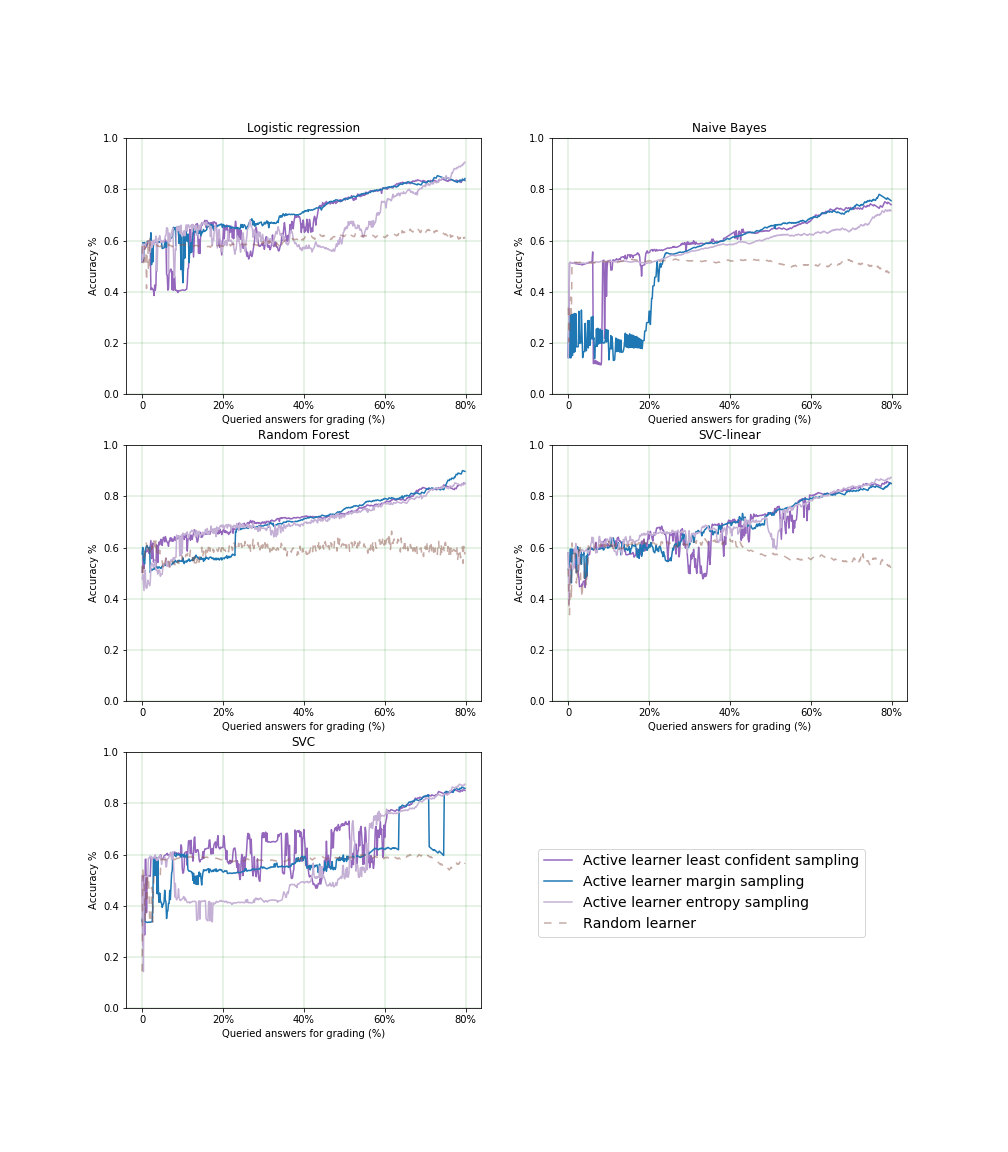
\includegraphics[scale=0.45]{images/task4_accuracy_uncertainty}
	\caption{Results in terms of accuracy for different models with uncertainty based query strategies.}
	\label{t4_m_uncertainty}
\end{figure}

\begin{figure}[!htb]
	\centering
	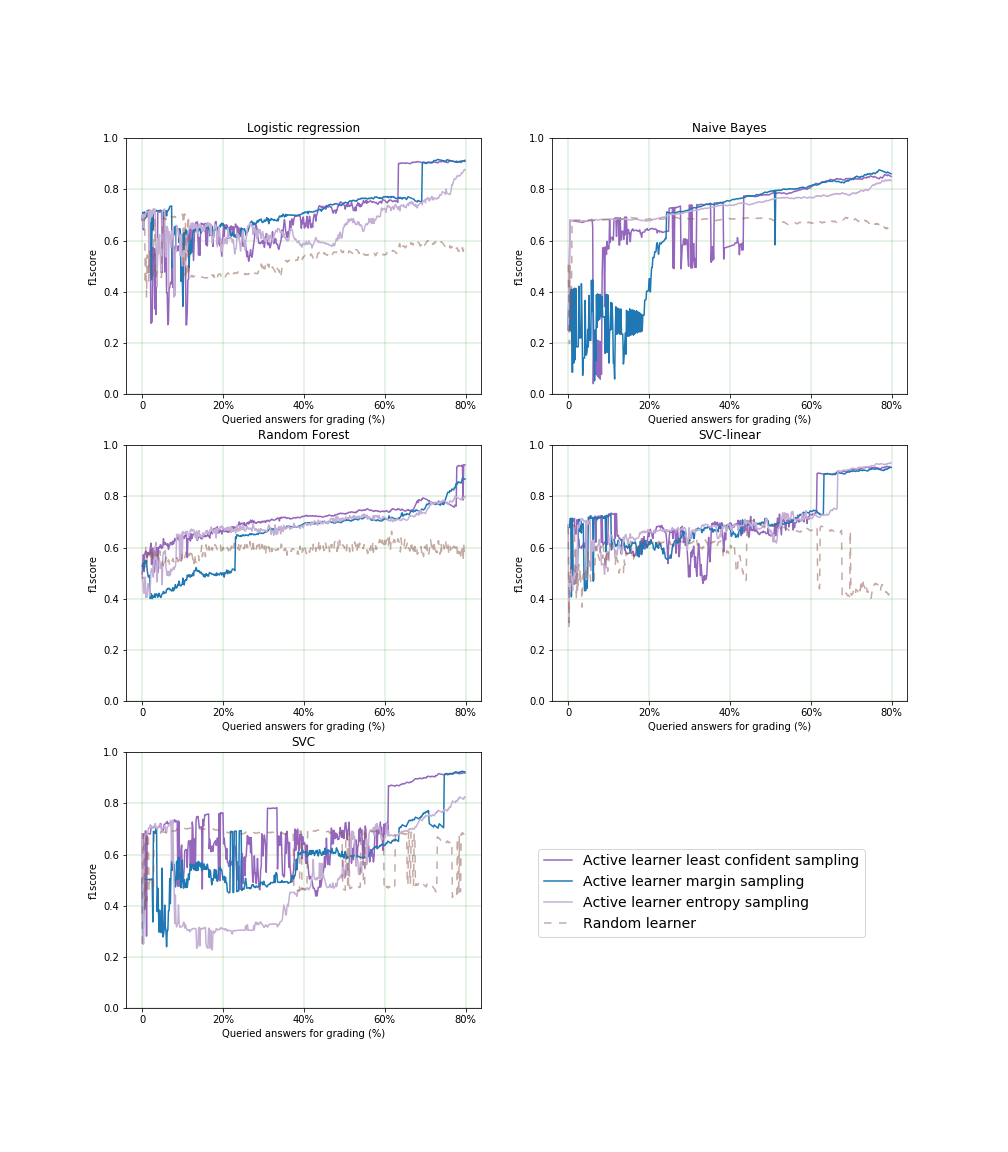
\includegraphics[scale=0.45]{images/task4_f1score_uncertainty}
	\caption{Results in terms of F1 score for different models with uncertainty based query strategies.}
	\label{t4_m_uncertainty_f1}
\end{figure}


\begin{figure}[!htb]
	\begin{subfigure}[b]{0.5\textwidth}
		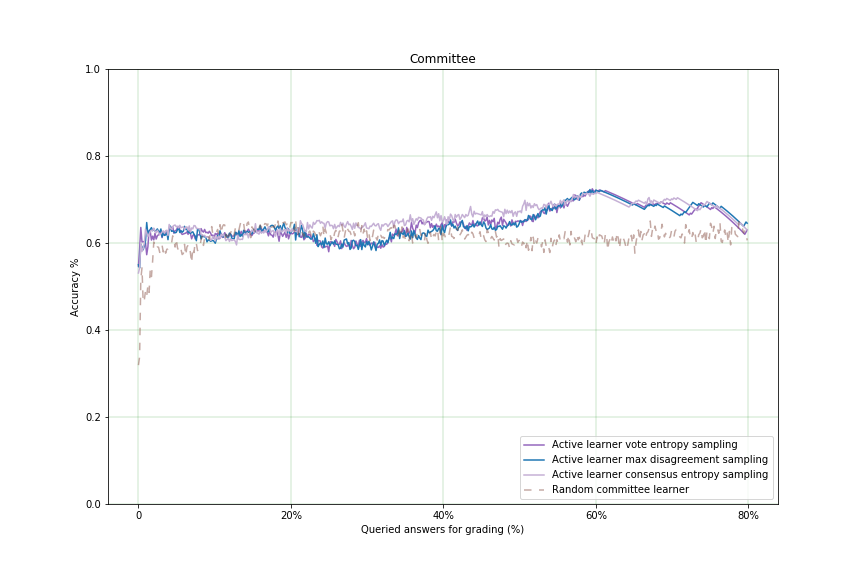
\includegraphics[width=\textwidth]{images/task4_accuracy_com}
		\caption{Results in terms of accuracy for committee based query strategies.}
		\label{t4_m_com}
	\end{subfigure}
	~
	\begin{subfigure}[b]{0.5\textwidth}
		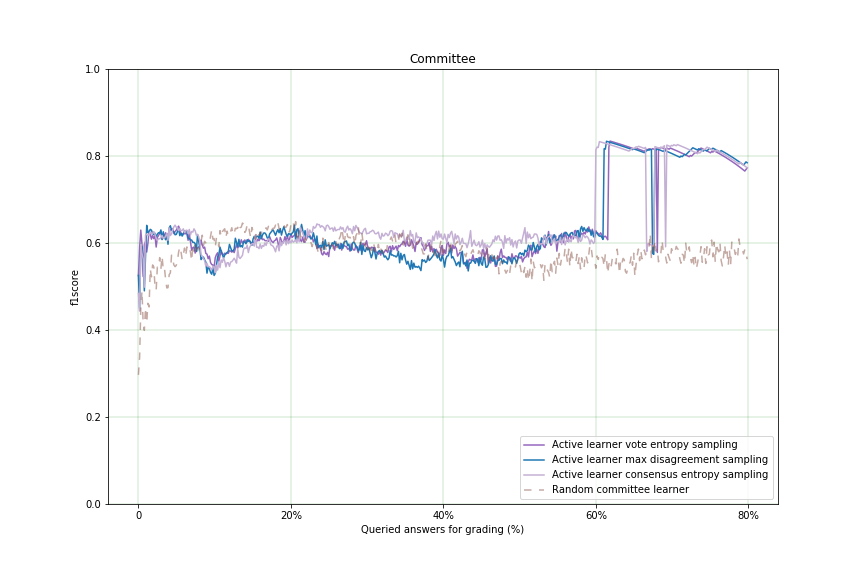
\includegraphics[width=\textwidth]{images/task4_f1score_com}
		\caption{Results in terms of F1 score for committee based query strategies.}
		\label{t4_m_com_f1}
	\end{subfigure}
	~
	\caption{Committee-based multi-class classification.}
\end{figure}

Taking the accuracy and the F1 scores into account, Logistic Regression with margin uncertainty sampling, Naive Bayes with least confident uncertainty sampling, Random Forest with least confident uncertainty sampling, and SVC-linear classifier with margin uncertainty sampling were selected for comparison using a bump chart Fig \ref{t4_m_bump}. The committee based query strategies didn't perform comparably to the uncertainty based query strategies and were ignored in the bump chart. The bump chart shows that the random forest with least confident sampling works well in the initial stages and after 45\% queries, logistic regression with margin sampling performs well. Hence, it could be inferred that both logistic regression and random forest work well for this dataset with Sultan'16 features.

\begin{figure}[h]
	\centering
	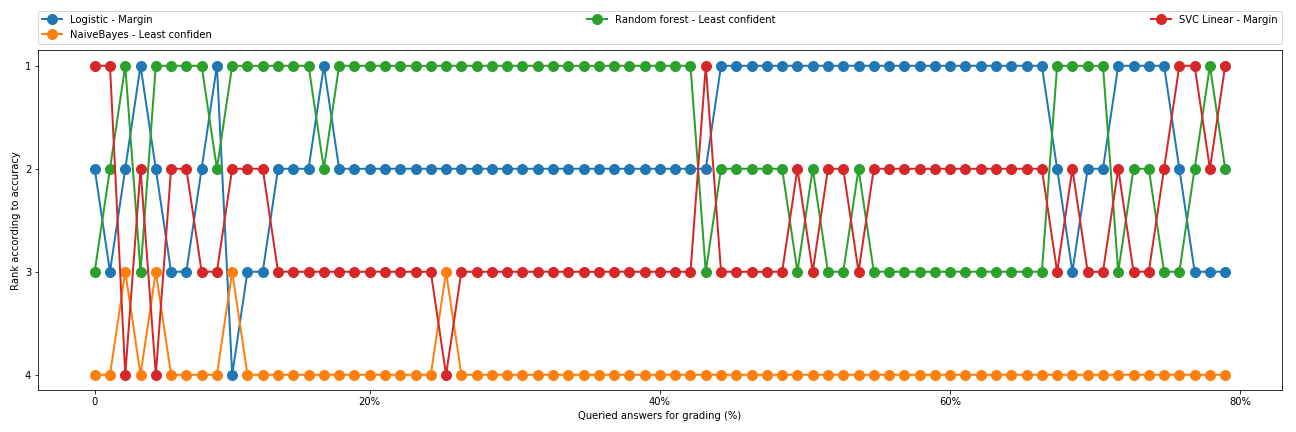
\includegraphics[scale=0.3]{images/task4_rank}
	\caption{Bump chart of model performance in multi-class classification.}
	\label{t4_m_bump}
\end{figure}



The time comparison of different models is tabulated in Table \ref{task4_m_time}. Considering the bump plot and the time comparison, it could be inferred that random forest classifier with least confident uncertainty sampling fits best for this setting. Though it takes approximately 0.3 seconds to process each query, that time would be negligible for the task of assisted-grading.

\begin{table}[!htb]
	\centering
	\scalebox{0.6}{
		\begin{tabular}{|c|c|c|c|c|c|c|}
			\hline
			& \multicolumn{6}{c|}{\textbf{Time taken per query (secs)}} \\ \hline
			\textbf{Models} & \textbf{\begin{tabular}[c]{@{}c@{}}least confident\\ uncertainty\end{tabular}} & \textbf{\begin{tabular}[c]{@{}c@{}}margin based \\ uncertainty\end{tabular}} & \textbf{\begin{tabular}[c]{@{}c@{}}entropy based \\ uncertainty\end{tabular}} & \textbf{\begin{tabular}[c]{@{}c@{}}vote \\ entropy\end{tabular}} & \textbf{\begin{tabular}[c]{@{}c@{}}max\\ disagreement\end{tabular}} & \textbf{\begin{tabular}[c]{@{}c@{}}consensus \\ entropy\end{tabular}} \\ \hline
			Logistic Regression & 0.0069 & 0.0070 & 0.0067 & \multirow{3}{*}{0.2169} & \multirow{3}{*}{0.2189} & \multirow{3}{*}{0.2150} \\ \cline{1-4}
			Naive Bayes & 0.0057 & 0.0060 & 0.0069 &  &  &  \\ \cline{1-4}
			\begin{tabular}[c]{@{}c@{}}Random Forest \\ (100 trees)\end{tabular} & 0.3407 & 0.3323 & 0.3028 &  &  &  \\ \hline
			SVC - Linear & 0.0206 & 0.0203 & 0.0216 & - & - & - \\ \hline
			SVC - RBF & 0.0473 & 0.0495 & 0.0444 & - & - & - \\ \hline
		\end{tabular}}
		\caption{Time comparison between different models for multi-class classification.}
		\label{task4_m_time}
	\end{table}
	
	%	Fig \ref{t1_m_best} shows the comparison between the performance of the best model in active learning setting and in a supervised learning setting with random splits.
	%	
	%	\begin{figure}[h]
	%		\centering
	%		\includegraphics[scale=0.35]{images/task1_best}
	%		\caption{Active vs. supervised learning for multi-class classification with Sultan'16 features.}
	%		\label{t1_m_best}
	%	\end{figure}		


% ======================= EX5 ==========================
\clearpage
\section{Experiment 5: Neural Network Dataset using Bag-of-words (BOW) Features}

Bag-of-words (BOW) of the answers were used as features for this experiment. Extracting this feature doesn't require reference answers of the questions as the entire BOW vectors were created from the student answers alone. Every answer was encoded into a vector of length 2540 and this vector was used as input to our models during training and prediction. The linear SVC and RBF kernel SVC models were ignored in this experiment as they consume a lot of time. Considering the future implementation of this project as an interactive task, time becomes a key factor to be considered.   

\subsection{Multi-class Classification}

The experimental results of different model-query strategy combinations in a multi-class classification setting are shown in Fig \ref{t5_m_uncertainty} and \ref{t5_m_com}. The results were also analyzed using the F1 score which are shown in Fig \ref{t5_m_uncertainty_f1} and Fig \ref{t5_m_com_f1}. The accuracy plots show that it is able to reach 70\% of accuracy with just 20\% queries in all the models. The accuracy improves with a small slope in the range of 25 - 80\% queries. It could be inferred from this that active learning is a better choice for this task as it performs well with less data. 

\begin{figure}[!htb]
	\centering
	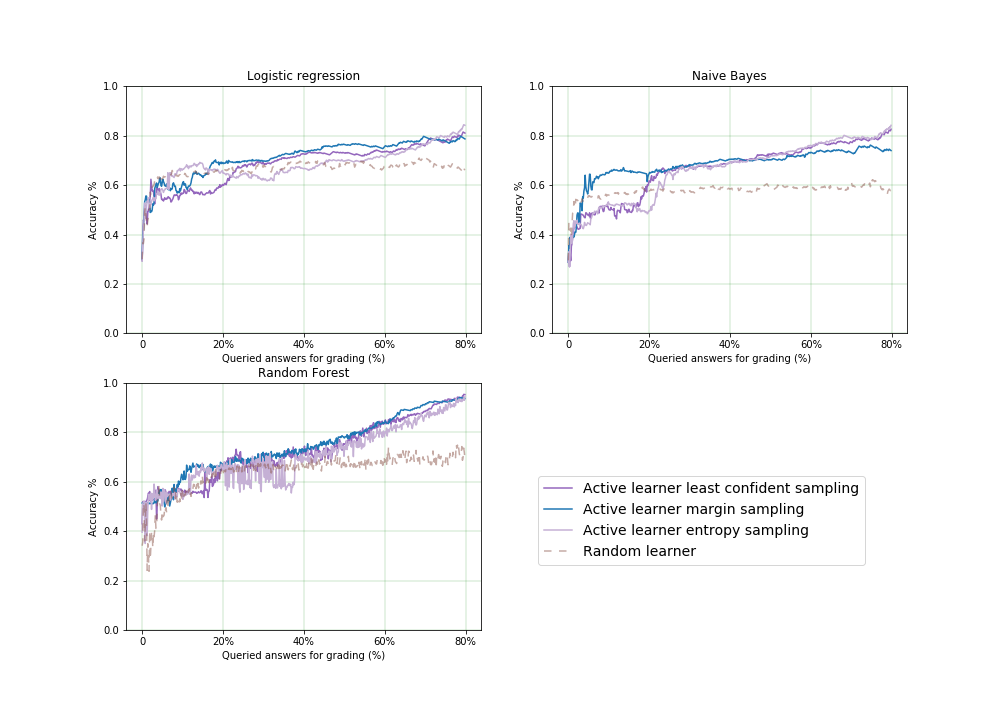
\includegraphics[scale=0.45]{images/task5_accuracy_uncertainty}
	\caption{Results in terms of accuracy for different models with uncertainty based query strategies.}
	\label{t5_m_uncertainty}
\end{figure}

\begin{figure}[!htb]
	\centering
	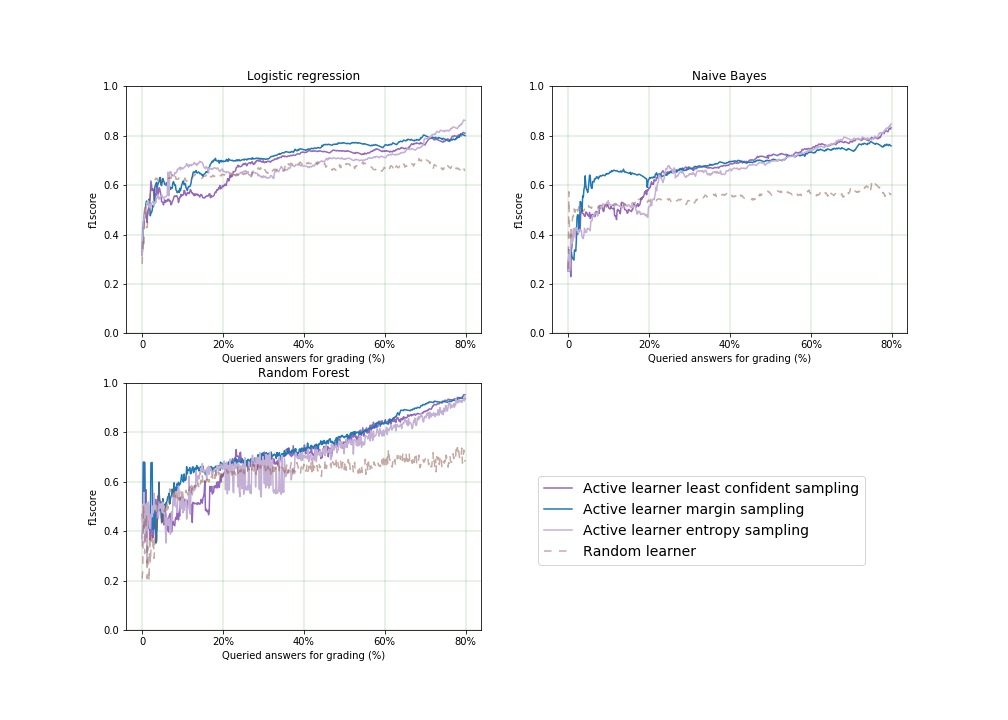
\includegraphics[scale=0.45]{images/task5_f1score_uncertainty}
	\caption{Results in terms of F1 score for different models with uncertainty based query strategies.}
	\label{t5_m_uncertainty_f1}
\end{figure}


\begin{figure}[!htb]
	\begin{subfigure}[b]{0.5\textwidth}
		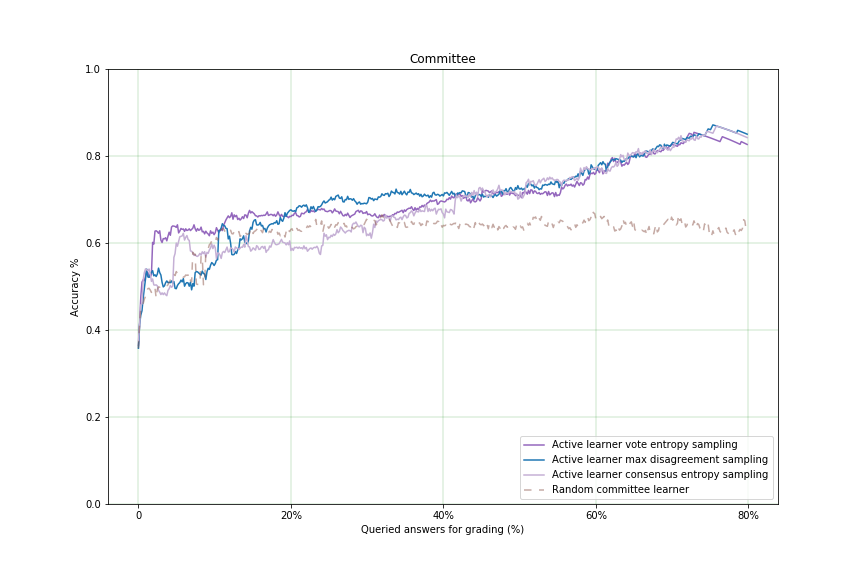
\includegraphics[width=\textwidth]{images/task5_accuracy_com}
		\caption{Results in terms of accuracy for committee based query strategies.}
		\label{t5_m_com}
	\end{subfigure}
	~
	\begin{subfigure}[b]{0.5\textwidth}
		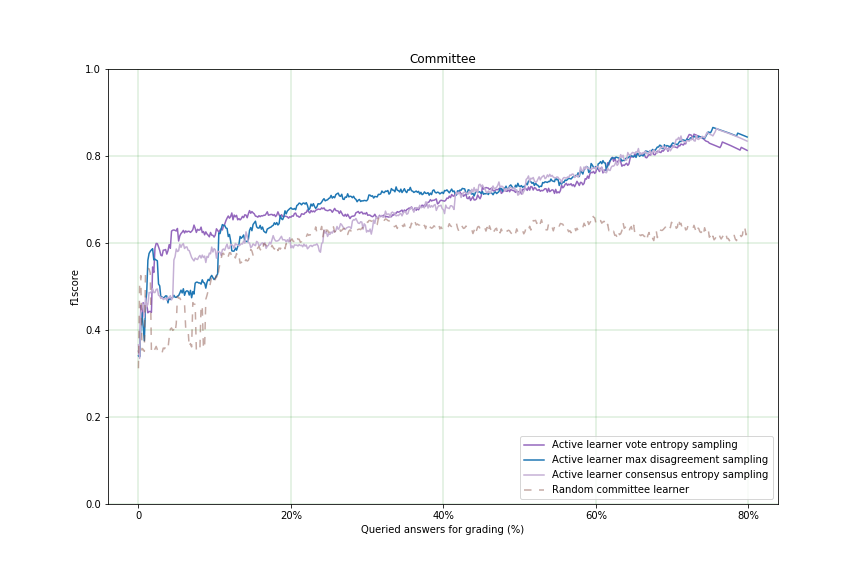
\includegraphics[width=\textwidth]{images/task5_f1score_com}
		\caption{Results in terms of F1 score for committee based query strategies.}
		\label{t5_m_com_f1}
	\end{subfigure}
	~
	\caption{Committee-based multi-class classification.}
\end{figure}

Considering the accuracy and the F1 scores, Logistic Regression with margin uncertainty sampling, Naive Bayes with least confident uncertainty sampling, and Random Forest with margin uncertainty sampling were selected for comparison using a bump chart Fig \ref{t5_m_bump}. In case of committee, max disagreement sampling performed better and is added to the bump chart comparison. The bump chart shows that the random forest classifier performs well over a long range.

\begin{figure}[t!]
	\centering
	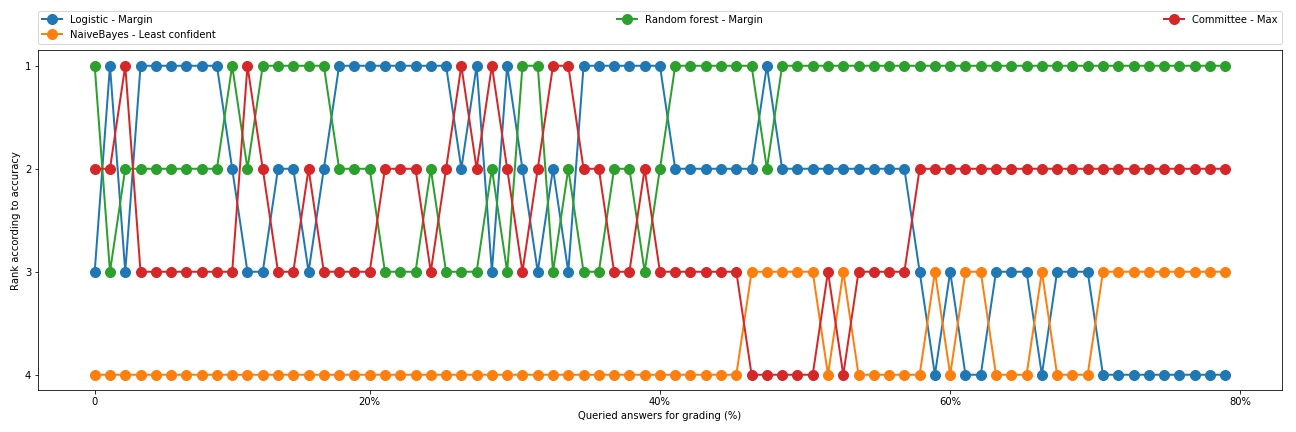
\includegraphics[scale=0.3]{images/task5_rank}
	\caption{Bump chart of model performance in multi-class classification.}
	\label{t5_m_bump}
	\vspace*{4.5in}
\end{figure}



The time comparison of different models is tabulated in Table \ref{task5_m_time}. Considering the bump plot and the time comparison, it could be inferred that random forest classifier with margin based uncertainty sampling fits best for this setting.

\begin{table}[!htb]
	\centering
	\scalebox{0.6}{
		\begin{tabular}{|c|c|c|c|c|c|c|}
			\hline
			& \multicolumn{6}{c|}{\textbf{Time taken per query (secs)}} \\ \hline
			\textbf{Models} & \textbf{\begin{tabular}[c]{@{}c@{}}least confident\\ uncertainty\end{tabular}} & \textbf{\begin{tabular}[c]{@{}c@{}}margin based \\ uncertainty\end{tabular}} & \textbf{\begin{tabular}[c]{@{}c@{}}entropy based \\ uncertainty\end{tabular}} & \textbf{\begin{tabular}[c]{@{}c@{}}vote \\ entropy\end{tabular}} & \textbf{\begin{tabular}[c]{@{}c@{}}max\\ disagreement\end{tabular}} & \textbf{\begin{tabular}[c]{@{}c@{}}consensus \\ entropy\end{tabular}} \\ \hline
			Logistic Regression & 0.0269 & 0.0261 & 0.0260 & \multirow{3}{*}{0.3481} & \multirow{3}{*}{0.3450} & \multirow{3}{*}{0.3276} \\ \cline{1-4}
			Naive Bayes & 0.0199 & 0.0187 & 0.0184 &  &  &  \\ \cline{1-4}
			\begin{tabular}[c]{@{}c@{}}Random Forest \\ (100 trees)\end{tabular} & 0.4545 & 0.4214 & 0.3952 &  &  &  \\ \hline
		\end{tabular}}
		\caption{Time comparison between different models for multi-class classification.}
		\label{task5_m_time}
	\end{table}
	
	%	Fig \ref{t1_m_best} shows the comparison between the performance of the best model in active learning setting and in a supervised learning setting with random splits.
	%	
	%	\begin{figure}[h]
	%		\centering
	%		\includegraphics[scale=0.35]{images/task1_best}
	%		\caption{Active vs. supervised learning for multi-class classification with Sultan'16 features.}
	%		\label{t1_m_best}
	%	\end{figure}
	
	% ======================= EX6 ==========================
	\clearpage
	\section{Experiment 6: Neural Network Dataset using Term Frequency-Inverse Document Frequency (tf-idf) Features}
	
	Neural Network dataset was experimented using term frequency-inverse document frequency (tf-idf) features.  Every answer was encoded into a vector of length 2540 and this vector was used as input to our models during training and prediction. Similar to the BOW features, tf-idf features also make up a huge feature space and thus, linear SVC and kernel based SVC were ignored in this experiment due to the time constraints.    
	
	\subsection{Multi-class Classification}
	
	The experimental results of different model-query strategy combinations in a multi-class classification setting are shown in Fig \ref{t6_m_uncertainty} and \ref{t6_m_com}. The results were also analyzed using the F1 score which are shown in Fig \ref{t6_m_uncertainty_f1} and Fig \ref{t6_m_com_f1}. 
	
	\begin{figure}[!htb]
		\centering
		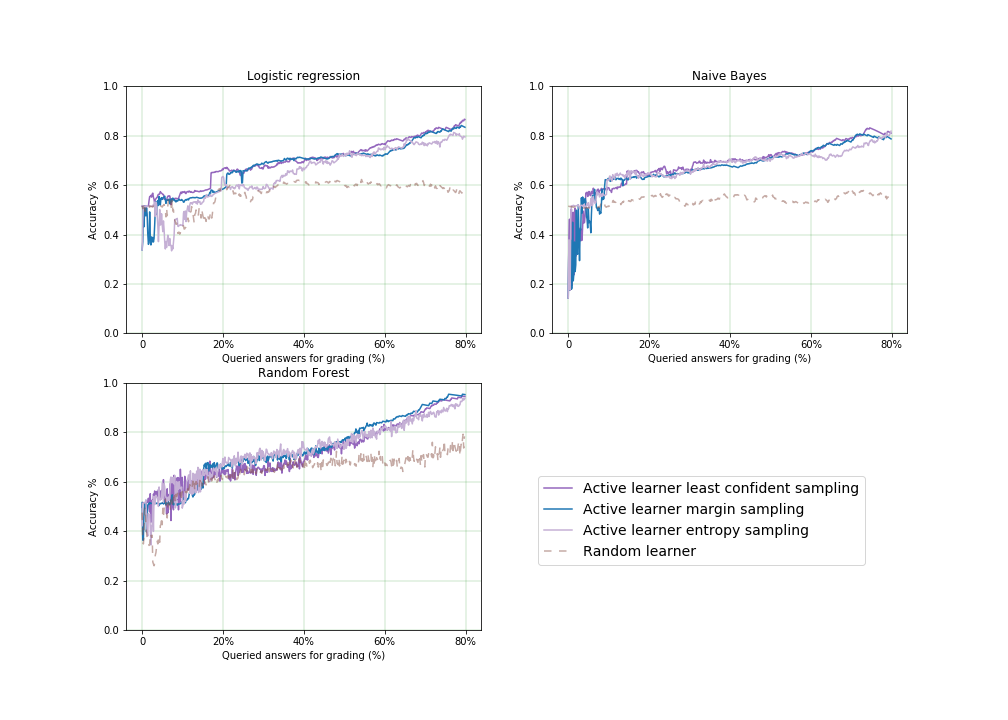
\includegraphics[scale=0.45]{images/task6_accuracy_uncertainty}
		\caption{Results in terms of accuracy for different models with uncertainty based query strategies.}
		\label{t6_m_uncertainty}
	\end{figure}
	
	\begin{figure}[!htb]
		\centering
		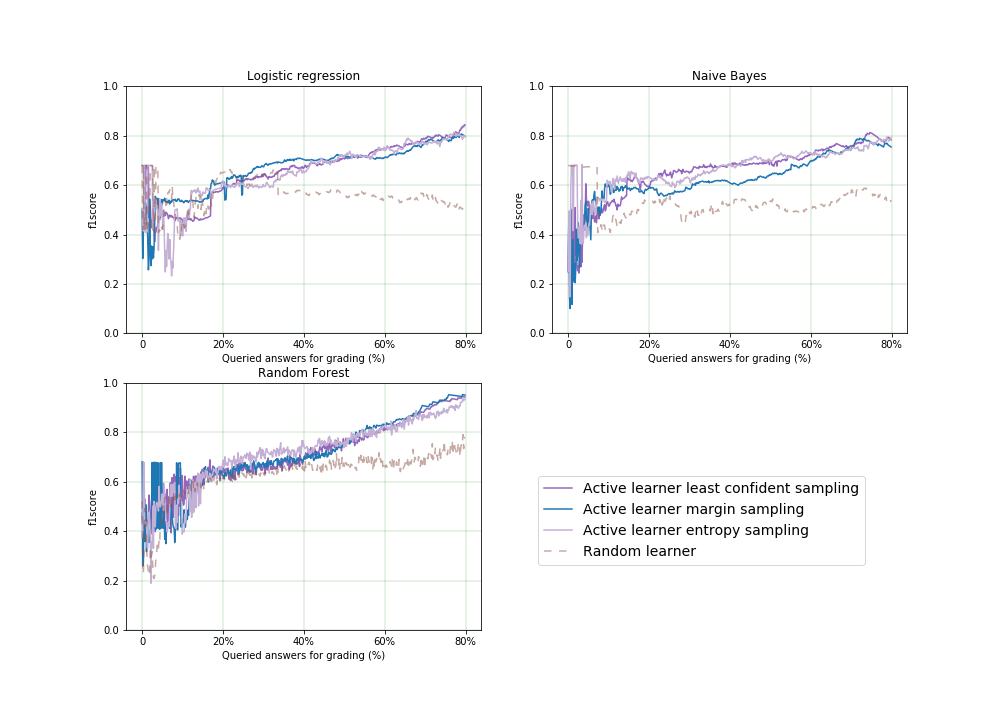
\includegraphics[scale=0.45]{images/task6_f1score_uncertainty}
		\caption{Results in terms of F1 score for different models with uncertainty based query strategies.}
		\label{t6_m_uncertainty_f1}
	\end{figure}
	
	
	\begin{figure}[!htb]
		\begin{subfigure}[b]{0.5\textwidth}
			\includegraphics[width=\textwidth]{images/task6_accuracy_com}
			\caption{Results in terms of accuracy for committee based query strategies.}
			\label{t6_m_com}
		\end{subfigure}
		~
		\begin{subfigure}[b]{0.5\textwidth}
			\includegraphics[width=\textwidth]{images/task6_f1score_com}
			\caption{Results in terms of F1 score for committee based query strategies.}
			\label{t6_m_com_f1}
		\end{subfigure}
		~
		\caption{Committee-based multi-class classification.}
	\end{figure}
	
	Considering the accuracy and the F1 scores, Logistic Regression with least confident uncertainty sampling, Naive Bayes with least confident uncertainty sampling, and Random Forest with margin uncertainty sampling were selected for comparison using a bump chart Fig \ref{t6_m_bump}. In case of committee, vote entropy sampling performed better and is added to the bump chart comparison. The bump chart shows that the random forest classifier clearly dominates over a long range. All the models perform comparably in the initial stages.
	
	\begin{figure}[h]
		\centering
		\includegraphics[scale=0.3]{images/task6_rank}
		\caption{Bump chart of model performance in multi-class classification.}
		\label{t6_m_bump}
	\end{figure}
	
	The time comparison of different models is tabulated in Table \ref{task6_m_time}. Considering the bump plot and the time comparison, it could be inferred that random forest classifier with margin based uncertainty sampling fits best for this setting.
	
	\begin{table}[!htb]
		\centering
		\scalebox{0.6}{
			\begin{tabular}{|c|c|c|c|c|c|c|}
				\hline
				& \multicolumn{6}{c|}{\textbf{Time taken per query (secs)}} \\ \hline
				\textbf{Models} & \textbf{\begin{tabular}[c]{@{}c@{}}least confident\\ uncertainty\end{tabular}} & \textbf{\begin{tabular}[c]{@{}c@{}}margin based \\ uncertainty\end{tabular}} & \textbf{\begin{tabular}[c]{@{}c@{}}entropy based \\ uncertainty\end{tabular}} & \textbf{\begin{tabular}[c]{@{}c@{}}vote \\ entropy\end{tabular}} & \textbf{\begin{tabular}[c]{@{}c@{}}max\\ disagreement\end{tabular}} & \textbf{\begin{tabular}[c]{@{}c@{}}consensus \\ entropy\end{tabular}} \\ \hline
				Logistic Regression & 0.0395 & 0.0388 & .0399 & \multirow{3}{*}{1.0785} & \multirow{3}{*}{1.0671} & \multirow{3}{*}{1.0725} \\ \cline{1-4}
				Naive Bayes & 0.0245 & 0.0243 & 0.0249 &  &  &  \\ \cline{1-4}
				\begin{tabular}[c]{@{}c@{}}Random Forest \\ (100 trees)\end{tabular} & 0.9430 & 0.9340 & 0.9538 &  &  &  \\ \hline
			\end{tabular}}
			\caption{Time comparison between different models for multi-class classification.}
			\label{task6_m_time}
		\end{table}
		
		%	Fig \ref{t1_m_best} shows the comparison between the performance of the best model in active learning setting and in a supervised learning setting with random splits.
		%	
		%	\begin{figure}[h]
		%		\centering
		%		\includegraphics[scale=0.35]{images/task1_best}
		%		\caption{Active vs. supervised learning for multi-class classification with Sultan'16 features.}
		%		\label{t1_m_best}
		%	\end{figure}	
		
\section{Experiment 7: SemEval Dataset using Features from Sultan'16}

Sultan'16 features were used in this experiment. The task of grading was split into binary classification and multi-class classification. The objective of binary classification is to identify correct and incorrect answers whereas multi-class classification's objective is to assign the correct grade for each answer. 

\subsection{Binary Classification}

The experimental results of different model-query strategy combinations in a binary classification setting are shown in Fig \ref{t7_b_uncertainty} and \ref{t7_b_com}. As the class distribution of this dataset is uneven, accuracy alone would not be enough to judge the performance of the models. Hence, the results were also analyzed using the F1 score which are shown in Fig \ref{t7_b_uncertainty_f1} and Fig \ref{t7_b_com_f1}.

\begin{figure}[!htb]
	\centering
	\includegraphics[scale=0.46]{images/binary/task7_accuracy_uncertainty}
	\caption{Results in terms of accuracy for different models with uncertainty based query strategies.}
	\label{t7_b_uncertainty}
\end{figure}

\begin{figure}[!htb]
	\centering
	\includegraphics[scale=0.46]{images/binary/task7_f1score_uncertainty}
	\caption{Results in terms of F1 score for different models with uncertainty based query strategies.}
	\label{t7_b_uncertainty_f1}
\end{figure}


\begin{figure}[!htb]
	\begin{subfigure}[b]{0.5\textwidth}
		\includegraphics[width=\textwidth]{images/binary/task7_accuracy_com}
		\caption{Results in terms of accuracy for committee based query strategies.}
		\label{t7_b_com}
	\end{subfigure}
	~
	\begin{subfigure}[b]{0.5\textwidth}
		\includegraphics[width=\textwidth]{images/binary/task7_f1score_com}
		\caption{Results in terms of F1 score for committee based query strategies.}
		\label{t7_b_com_f1}
	\end{subfigure}
	~
	\caption{Committee-based binary classification.}
\end{figure}

Based on these graphs, we observe that all the active learning query strategies outperform the passive learning. We also observe that all the active learning strategies in their respective models performed comparably to each other. Hence, we selected the margin based uncertainty sampling for each model in order to compare them using a bump chart. This chart shows the performance of every model ranked by their accuracies which is shown in Fig \ref{t7_b_bump}. The bump chart for binary classification shows that all logistic regression with margin uncertainty sampling works well for this setting, and is a clear winner performing consistently better over a long range. 

\begin{figure}[!htb]
	\centering
	\includegraphics[scale=0.3]{images/binary/task7_rank}
	\caption{Bump chart of model performance in binary classification.}
	\label{t7_b_bump}
\end{figure}



%	Fig \ref{t1_b_best} shows the comparison between the performance of the best model in active learning setting and in a supervised learning setting with random splits.
%	
%	\begin{figure}[!htb]
%		\centering
%		\includegraphics[scale=0.35]{images/binary/task1_best}
%		\caption{Active vs. supervised learning for binary classification with Sultan'16 features.}
%		\label{t1_b_best}
%	\end{figure}



%================================================
\clearpage
\subsection{Multi-class Classification}

The experimental results of different model-query strategy combinations in a multi-class classification setting are shown in Fig \ref{t7_m_uncertainty} and \ref{t7_m_com}. The results were also analyzed using the F1 score which are shown in Fig \ref{t7_m_uncertainty_f1} and Fig \ref{t7_m_com_f1}.

\begin{figure}[!htb]
	\centering
	\includegraphics[scale=0.45]{images/task7_accuracy_uncertainty}
	\caption{Results in terms of accuracy for different models with uncertainty based query strategies.}
	\label{t7_m_uncertainty}
\end{figure}

\begin{figure}[!htb]
	\centering
	\includegraphics[scale=0.45]{images/task7_f1score_uncertainty}
	\caption{Results in terms of F1 score for different models with uncertainty based query strategies.}
	\label{t7_m_uncertainty_f1}
\end{figure}


\begin{figure}[!htb]
	\begin{subfigure}[b]{0.5\textwidth}
		\includegraphics[width=\textwidth]{images/task7_accuracy_com}
		\caption{Results in terms of accuracy for committee based query strategies.}
		\label{t7_m_com}
	\end{subfigure}
	~
	\begin{subfigure}[b]{0.5\textwidth}
		\includegraphics[width=\textwidth]{images/task7_f1score_com}
		\caption{Results in terms of F1 score for committee based query strategies.}
		\label{t7_m_com_f1}
	\end{subfigure}
	~
	\caption{Committee-based multi-class classification.}
\end{figure}

We observe that all the active learning query strategies outperform the passive learning (random sampling). Considering the accuracy and the F1 scores, logistic regression with margin uncertainty sampling, naive Bayes with margin uncertainty sampling, random forest with margin uncertainty sampling, and linear SVM with least confident uncertainty sampling were selected for comparison using a bump chart. In case of committee, max disagreement sampling performed better and is added to the bump chart comparison. This chart shows the performance of every model ranked by their accuracies which is shown in Fig \ref{t7_m_bump}.

\begin{figure}[h]
	\centering
	\includegraphics[scale=0.3]{images/task7_rank}
	\caption{Bump chart of model performance in multi-class classification.}
	\label{t7_m_bump}
\end{figure}

The bump chart shows that the random forest classifier model with margin uncertainty sampling and logistic regression classifier with margin uncertainty sampling are preferable for this setting. Random forest classifier shows consistent and good performance after 40\% of the queries. 

The time comparison of different models is tabulated in Table \ref{task7_m_time}. Based on the bump plot and time comparison, it could be inferred that random forest with least confident uncertainty sampling is best for SemEval 2013 dataset with Sultan'16 features.  

\begin{table}[!htb]
	\centering
	\scalebox{0.6}{
		\begin{tabular}{|c|c|c|c|c|c|c|}
			\hline
			& \multicolumn{6}{c|}{\textbf{Time taken per query (secs)}} \\ \hline
			\textbf{Models} & \textbf{\begin{tabular}[c]{@{}c@{}}least confident\\ uncertainty\end{tabular}} & \textbf{\begin{tabular}[c]{@{}c@{}}margin based \\ uncertainty\end{tabular}} & \textbf{\begin{tabular}[c]{@{}c@{}}entropy based \\ uncertainty\end{tabular}} & \textbf{\begin{tabular}[c]{@{}c@{}}vote \\ entropy\end{tabular}} & \textbf{\begin{tabular}[c]{@{}c@{}}max\\ disagreement\end{tabular}} & \textbf{\begin{tabular}[c]{@{}c@{}}consensus \\ entropy\end{tabular}} \\ \hline
			Logistic Regression & 0.0530 & 0.0506 & 0.0519 & \multirow{3}{*}{0.8570} & \multirow{3}{*}{0.8132} & \multirow{3}{*}{0.8008} \\ \cline{1-4}
			Naive Bayes & 0.0217 & 0.0199 & 0.0217 &  &  &  \\ \cline{1-4}
			\begin{tabular}[c]{@{}c@{}}Random Forest \\ (100 trees)\end{tabular} & 0.7391 & 0.5579 & 0.5538 &  &  &  \\ \hline
			SVC Linear & 0.6159 & 0.5972 & 0.6064 & - & - & - \\ \hline
			SVC RBF & 1.9078 & 1.8223 & 1.9001 & - & - & - \\ \hline
		\end{tabular}}
		\caption{Time comparison between different models for multi-class classification.}
		\label{task7_m_time}
	\end{table}
	
	%	Fig \ref{t1_m_best} shows the comparison between the performance of the best model in active learning setting and in a supervised learning setting with random splits.
	%	
	%	\begin{figure}[h]
	%		\centering
	%		\includegraphics[scale=0.35]{images/task1_best}
	%		\caption{Active vs. supervised learning for multi-class classification with Sultan'16 features.}
	%		\label{t1_m_best}
	%	\end{figure}
	
	\clearpage
	
%======================= EX8 ==============================
\section{Experiment 8: SemEval 2013 Dataset using Bag-of-words (BOW) Features}

Bag-of-words(BOW) of the answers were used as features for this experiment. Extracting this feature doesn't require reference answers of the questions as the entire BOW vectors were created from the student answers alone. Every answer was encoded into a vector of length 1908 and this vector was used as input to our models during training and prediction. The linear SVC and RBF kernel SVC models were ignored in this experiment as they consume a lot of time to select each query since the dimension of the feature space is very high. Considering the future implementation of this project as an interactive task, time becomes a key factor to be considered.   

\subsection{Binary Classification}

The experimental results of different model-query strategy combinations in a binary classification setting are shown in Fig \ref{t8_b_uncertainty} and \ref{t8_b_com}. The F1 score analysis of this experiment is shown in Fig \ref{t8_b_uncertainty_f1} and Fig \ref{t8_b_com_f1}. 

\begin{figure}[!htb]
	\centering
	\includegraphics[scale=0.46]{images/binary/task8_accuracy_uncertainty}
	\caption{Results in terms of accuracy for different models with uncertainty based query strategies.}
	\label{t8_b_uncertainty}
\end{figure}

\begin{figure}[!htb]
	\centering
	\includegraphics[scale=0.46]{images/binary/task8_f1score_uncertainty}
	\caption{Results in terms of F1 score for different models with uncertainty based query strategies.}
	\label{t8_b_uncertainty_f1}
\end{figure}


\begin{figure}[!htb]
	\begin{subfigure}[b]{0.5\textwidth}
		\includegraphics[width=\textwidth]{images/binary/task8_accuracy_com}
		\caption{Results in terms of accuracy for committee based query strategies.}
		\label{t8_b_com}
	\end{subfigure}
	~
	\begin{subfigure}[b]{0.5\textwidth}
		\includegraphics[width=\textwidth]{images/binary/task8_f1score_com}
		\caption{Results in terms of F1 score for committee based query strategies.}
		\label{t8_b_com_f1}
	\end{subfigure}
	~
	\caption{Committee-based binary classification.}
\end{figure}

We observe that all the active learning strategies in their respective models performed comparably to each other. Hence, we selected the margin uncertainty sampling for the random forest and logistic regression models, entropy uncertainty for naive Bayes classifier, and vote entropy sampling for the committee based model to have a closer look at their performance over increasing number of queries using a bump chart. This chart shows the performance of every model ranked by their accuracies which is shown in Fig \ref{t8_b_bump}.

\begin{figure}[!htb]
	\includegraphics[scale=0.3]{images/binary/task8_rank}
	\caption{Bump chart of model performance in binary classification.}
	\label{t8_b_bump}
\end{figure}


We can infer from the bump chart that the random forest with margin uncertainty sampling performs well in the overall range. When considering the overall chart, it seems wise to select random forest classifier with margin based sampling for this setting. 

%	Fig \ref{t1_b_best} shows the comparison between the performance of the best model in active learning setting and in a supervised learning setting with random splits.
%	
%	\begin{figure}[!htb]
%		\centering
%		\includegraphics[scale=0.35]{images/binary/task1_best}
%		\caption{Active vs. supervised learning for binary classification with Sultan'16 features.}
%		\label{t1_b_best}
%	\end{figure}



%================================================
\clearpage
\subsection{Multi-class Classification}

The experimental results of different model-query strategy combinations in a multi-class classification setting are shown in Fig \ref{t8_m_uncertainty} and \ref{t8_m_com}. The results were also analyzed using the F1 score which are shown in Fig \ref{t8_m_uncertainty_f1} and Fig \ref{t8_m_com_f1}.

\begin{figure}[!htb]
	\centering
	\includegraphics[scale=0.45]{images/task8_accuracy_uncertainty}
	\caption{Results in terms of accuracy for different models with uncertainty based query strategies.}
	\label{t8_m_uncertainty}
\end{figure}

\begin{figure}[!htb]
	\centering
	\includegraphics[scale=0.45]{images/task8_f1score_uncertainty}
	\caption{Results in terms of F1 score for different models with uncertainty based query strategies.}
	\label{t8_m_uncertainty_f1}
\end{figure}


\begin{figure}[!htb]
	\begin{subfigure}[b]{0.5\textwidth}
		\includegraphics[width=\textwidth]{images/task8_accuracy_com}
		\caption{Results in terms of accuracy for committee based query strategies.}
		\label{t8_m_com}
	\end{subfigure}
	~
	\begin{subfigure}[b]{0.5\textwidth}
		\includegraphics[width=\textwidth]{images/task8_f1score_com}
		\caption{Results in terms of F1 score for committee based query strategies.}
		\label{t8_m_com_f1}
	\end{subfigure}
	~
	\caption{Committee-based multi-class classification.}
\end{figure}

Considering the accuracy and the F1 scores, Logistic Regression with margin uncertainty sampling, Naive Bayes with margin uncertainty sampling, and Random Forest with least confident uncertainty sampling were selected for comparison using a bump chart. In case of committee, max disagreement sampling performed better and is added to the bump chart Fig \ref{t8_m_bump} comparison. The bump chart shows that the logistic regression classifier and random forest perform compably to each other. Logistic regression performs well during the first half queries and random forest performs well during the last stages.

\begin{figure}[h]
	\centering
	\includegraphics[scale=0.3]{images/task8_rank}
	\caption{Bump chart of model performance in multi-class classification.}
	\label{t8_m_bump}
\end{figure}





		\begin{table}[!htb]
			\centering
			\scalebox{0.6}{
				\begin{tabular}{|c|c|c|c|c|c|c|}
		\hline
		& \multicolumn{6}{c|}{\textbf{Time taken per query (secs)}} \\ \hline
		\textbf{Models} & \textbf{\begin{tabular}[c]{@{}c@{}}least confident\\ uncertainty\end{tabular}} & \textbf{\begin{tabular}[c]{@{}c@{}}margin based \\ uncertainty\end{tabular}} & \textbf{\begin{tabular}[c]{@{}c@{}}entropy based \\ uncertainty\end{tabular}} & \textbf{\begin{tabular}[c]{@{}c@{}}vote \\ entropy\end{tabular}} & \textbf{\begin{tabular}[c]{@{}c@{}}max\\ disagreement\end{tabular}} & \textbf{\begin{tabular}[c]{@{}c@{}}consensus \\ entropy\end{tabular}} \\ \hline
		Logistic Regression & 0.2076 & 0.1573 & 0.1423 & \multirow{3}{*}{3.7620} & \multirow{3}{*}{3.5757} & \multirow{3}{*}{3.5843} \\ \cline{1-4}
		Naive Bayes & 0.0938 & 0.0915 & 0.0910 &  &  &  \\ \cline{1-4}
		\begin{tabular}[c]{@{}c@{}}Random Forest \\ (100 trees)\end{tabular} & 3.4522 & 3.3247 & 3.1755 &  &  &  \\ \hline
		\end{tabular}}
		\caption{Time comparison between different models for multi-class classification.}
		\label{task8_m_time}
	\end{table}
	
	
	The time comparison of different models is tabulated in Table \ref{task8_m_time}. Considering the bump plot and the time comparison, it could be inferred that logistic regression classifier with margin based uncertainty sampling fits best for this setting as random forest takes more than 3 seconds for every query which is a long waiting time in a practical application.
	
	%	Fig \ref{t1_m_best} shows the comparison between the performance of the best model in active learning setting and in a supervised learning setting with random splits.
	%	
	%	\begin{figure}[h]
	%		\centering
	%		\includegraphics[scale=0.35]{images/task1_best}
	%		\caption{Active vs. supervised learning for multi-class classification with Sultan'16 features.}
	%		\label{t1_m_best}
	%	\end{figure}
	
\clearpage
%========================== EX9 ===============================

\section{Experiment 9: SemEval 2013 Dataset using Term Frequency-Inverse Document Frequency (tf-idf) Features}

In this experiment, the SemEval dataset was experimented using term frequency-inverse document frequency (tf-idf) features. Every answer was encoded into a vector of length 1908 and this vector was used as input to our models during training and prediction. Similar to the BOW features, tf-idf features also make up a huge feature space and thus, linear SVC and kernel based SVC were ignored in this experiment due to the time constraints.    

\subsection{Binary Classification}

The experimental results of different model-query strategy combinations in a binary classification setting are shown in Fig \ref{t9_b_uncertainty} and \ref{t9_b_com}. The F1 score analysis of this experiment is shown in Fig \ref{t9_b_uncertainty_f1} and Fig \ref{t9_b_com_f1}. 

\begin{figure}[!htb]
	\centering
	\includegraphics[scale=0.46]{images/binary/task9_accuracy_uncertainty}
	\caption{Results in terms of accuracy for different models with uncertainty based query strategies.}
	\label{t9_b_uncertainty}
\end{figure}

\begin{figure}[!htb]
	\centering
	\includegraphics[scale=0.46]{images/binary/task9_f1score_uncertainty}
	\caption{Results in terms of F1 score for different models with uncertainty based query strategies.}
	\label{t9_b_uncertainty_f1}
\end{figure}


\begin{figure}[!htb]
	\begin{subfigure}[b]{0.5\textwidth}
		\includegraphics[width=\textwidth]{images/binary/task9_accuracy_com}
		\caption{Results in terms of accuracy for committee based query strategies.}
		\label{t9_b_com}
	\end{subfigure}
	~
	\begin{subfigure}[b]{0.5\textwidth}
		\includegraphics[width=\textwidth]{images/binary/task9_f1score_com}
		\caption{Results in terms of F1 score for committee based query strategies.}
		\label{t9_b_com_f1}
	\end{subfigure}
	~
	\caption{Committee-based binary classification.}
\end{figure}

We observe that all the active learning strategies in their respective models performed comparably to each other. Hence, we selected the margin uncertainty sampling for the naive Bayes, logistic regression, and random forest classifier models to have a closer look at their performance over increasing number of queries using a bump chart Fig \ref{t9_b_bump}. Logistic regression classifier performs well initially and random forest performs well after 35\% of the queries.  

\begin{figure}[!htb]
	\includegraphics[scale=0.3]{images/binary/task9_rank}
	\caption{Bump chart of model performance in binary classification.}
	\label{t9_b_bump}
\end{figure}


%	Fig \ref{t1_b_best} shows the comparison between the performance of the best model in active learning setting and in a supervised learning setting with random splits.
%	
%	\begin{figure}[!htb]
%		\centering
%		\includegraphics[scale=0.35]{images/binary/task1_best}
%		\caption{Active vs. supervised learning for binary classification with Sultan'16 features.}
%		\label{t1_b_best}
%	\end{figure}



%================================================
\clearpage
\subsection{Multi-class Classification}

The experimental results of different model-query strategy combinations in a multi-class classification setting are shown in Fig \ref{t9_m_uncertainty} and \ref{t9_m_com}. The results were also analyzed using the F1 score which are shown in Fig \ref{t9_m_uncertainty_f1} and Fig \ref{t9_m_com_f1}.

\begin{figure}[!htb]
	\centering
	\includegraphics[scale=0.45]{images/task9_accuracy_uncertainty}
	\caption{Results in terms of accuracy for different models with uncertainty based query strategies.}
	\label{t9_m_uncertainty}
\end{figure}

\begin{figure}[!htb]
	\centering
	\includegraphics[scale=0.45]{images/task9_f1score_uncertainty}
	\caption{Results in terms of F1 score for different models with uncertainty based query strategies.}
	\label{t9_m_uncertainty_f1}
\end{figure}


\begin{figure}[!htb]
	\begin{subfigure}[b]{0.5\textwidth}
		\includegraphics[width=\textwidth]{images/task9_accuracy_com}
		\caption{Results in terms of accuracy for committee based query strategies.}
		\label{t9_m_com}
	\end{subfigure}
	~
	\begin{subfigure}[b]{0.5\textwidth}
		\includegraphics[width=\textwidth]{images/task9_f1score_com}
		\caption{Results in terms of F1 score for committee based query strategies.}
		\label{t9_m_com_f1}
	\end{subfigure}
	~
	\caption{Committee-based multi-class classification.}
\end{figure}

Considering the accuracy and the F1 scores, Logistic Regression with margin uncertainty sampling, Naive Bayes with margin uncertainty sampling, and Random Forest with margin uncertainty sampling were selected for comparison using a bump chart. In case of committee, max disagreement sampling performed better and is added to the bump chart comparison. This chart shows the performance of every model ranked by their accuracies which is shown in Fig \ref{t9_m_bump}. The bump chart shows that the committee of models and logistic regression models perform comparable to each other over the whole range of queries.

\begin{figure}[h]
	\centering
	\includegraphics[scale=0.3]{images/task9_rank}
	\caption{Bump chart of model performance in multi-class classification.}
	\label{t9_m_bump}
\end{figure}



The time comparison of different models is tabulated in Table \ref{task9_m_time}. Considering the bump plot and the time comparison, it could be inferred that logistic regression classifier with margin based uncertainty sampling fits best for this setting. Committee based learning is ignored as it takes a lot of time.

	\begin{table}[!htb]
		\centering
		\scalebox{0.6}{
			\begin{tabular}{|c|c|c|c|c|c|c|}
			\hline
			& \multicolumn{6}{c|}{\textbf{Time taken per query (secs)}} \\ \hline
			\textbf{Models} & \textbf{\begin{tabular}[c]{@{}c@{}}least confident\\ uncertainty\end{tabular}} & \textbf{\begin{tabular}[c]{@{}c@{}}margin based \\ uncertainty\end{tabular}} & \textbf{\begin{tabular}[c]{@{}c@{}}entropy based \\ uncertainty\end{tabular}} & \textbf{\begin{tabular}[c]{@{}c@{}}vote \\ entropy\end{tabular}} & \textbf{\begin{tabular}[c]{@{}c@{}}max\\ disagreement\end{tabular}} & \textbf{\begin{tabular}[c]{@{}c@{}}consensus \\ entropy\end{tabular}} \\ \hline
			Logistic Regression & 0.1322 & 0.1121 & 0.0997 & \multirow{3}{*}{4.0031} & \multirow{3}{*}{3.7025} & \multirow{3}{*}{3.6239} \\ \cline{1-4}
			Naive Bayes & 0.0630 & 0.0612 & 0.0627 &  &  &  \\ \cline{1-4}
			\begin{tabular}[c]{@{}c@{}}Random Forest \\ (100 trees)\end{tabular} & 3.6896 & 3.5362 & 3.3289 &  &  &  \\ \hline
			\end{tabular}}
		\caption{Time comparison between different models for multi-class classification.}
		\label{task9_m_time}
	\end{table}
	
%		Fig \ref{t1_m_best} shows the comparison between the performance of the best model in active learning setting and in a supervised learning setting with random splits.
%		
%		\begin{figure}[h]
%			\centering
%			\includegraphics[scale=0.35]{images/task1_best}
%			\caption{Active vs. supervised learning for multi-class classification with Sultan'16 features.}
%			\label{t1_m_best}
%		\end{figure}

\clearpage
%=================== Batch size comparison ========================

\section{Experiment 10: Influence of seed and batch size}

Batch size is one of the important setting which influences the performance of active learning. To evaluate the effectiveness of different batch sizes, the active learning setting that performed best on the previous experiments on the SemEval 2013 dataset was used in this experiment. Random forest model consisting of 100 trees with least confident uncertainty sampling was trained on 40\% of SemEval's train dataset and then this model is used to evaluate the performance on the students' answers. The active learning is done with varying batch sizes and the accuracy on unseen answers test set have been tabulated in table \ref{batch_comparison}.

\begin{table}[!htb]
	\centering
	\scalebox{0.9}{
		\begin{tabular}{|c|c|c|c|c|c|c|c|}
			\hline
			\textbf{Batch Size} & 1  & 3     & 5     & 7     & 10    & 20    & 50    \\ \hline
			\textbf{Accuracy}   & \textbf{0.537} & 0.492 & 0.505 & 0.494 & 0.511 & 0.516 & 0.518 \\ \hline
		\end{tabular}}
		\caption{Accuracy for different batch sizes.}
		\label{batch_comparison}
	\end{table}
	
We can infer that querying the human expert the grades for one question at a time yields more accuracy than using higher batch sizes. The reason behind this could be that active learning choses samples from different regions in the sample space while querying one by one which in turns helps it to fix a better decision boundary between the classes. In contrast, querying in batches of size more than one may try to query samples from the same neighborhood which results in its poor performance \cite{Horbach2016}. 

Seeding is another important aspect of active learning as it defines the samples from which to learn the model initially. Different strategies for seeding exists such as random seeding (randomly selecting the samples), one sample per class, and multiple samples per class. We opted for one sample per class in our experiments as work by Horbach et al \cite{Horbach2016}., claimed that equal seeding has more impact on the performance of the machine learning model. Though one sample per class could easily be obtained from an existing dataset, efficient methods to find the seeds would be a challenge for a new set of answers and questions. Clustering the sample space with the grades as cluster numbers and seeding one sample per cluster could be efficient in such a setting.  

	
\clearpage
%=================== Question-wise Comparison ========================

\section{Experiment 11: Question-wise analysis of the best setting.}

The best active learning setting based on the previous experiments on the SemEval 2013 dataset was used in this experiment to observe the model's performance on different questions. The random forest model consisting of 100 trees with least confident uncertainty sampling was trained on 20\% of SemEval's train dataset and then this model is used to evaluate the performance on the students' answers for every question. Fig \ref{sem_ques} shows the accuracy obtained on every question using this model.

 \begin{figure}[!htb]
	\centering
	\includegraphics[scale=0.41]{images/sem_ques}
	\caption{Accuracy obtained by active learning on every question of SemEval dataset.}
	\label{sem_ques}
\end{figure}

It can be seen from the graph that the model doesn't perform consistently on every question. Following are the questions and their reference answers for which the model achieved more than 90\% accuracy. 

\noindent \textbf{Question}: Andi and Scott decided to investigate solar water heaters using collectors of different colors (but the same size) as one variable and covered versus uncovered as a second variable. Look at the graph of their data and answer the questions below. What does the graph tell you about the effect of using a cover?

\noindent \textbf{Reference answer}: Water heats up faster when covered.

\vspace{5mm} 

\noindent \textbf{Question}: Paula wants to test a food to see if it contains acid and/or sugar. When Paula added water and yeast to a sample of the food and put the mixture in a warm water bath, the mixture began to fizz and bubble. What does this chemical reaction indicate?

\noindent \textbf{Reference answer}: The food contains sugar.

\vspace{5mm} 


The questions are of closed type where the answers are very short and decisive. The features used in this experiment are capable of capturing such answers which contain similar wordings as the reference answers of paraphrases of it. This could be a possible reason behind the better performance of this model on these questions.

\vspace{3mm} 

Following are the questions on which the model achieved less than 30\% of accuracy. 

\vspace{5mm} 


\noindent \textbf{Question}: The graph shows temperature data from 2 containers. One container had 100 milliliters of water and the other had 100 milliliters of dry soil. Each container was placed in the sun for 20 minutes and then in the shade for 20 minutes. Which container, A or B, had the dry soil? Explain how the graph helped you decide which container had the dry soil.

\noindent \textbf{Reference answer}: A. Dry soil heats more quickly and cools off more quickly than water. The graph shows A heats and cools more quickly than B, so A must be the dry soil.

\vspace{5mm}

\noindent \textbf{Question}: Denise made a circuit to light a bulb or run a motor. She used a special switch. Below is the schematic diagram of her circuit. The switch is inside the dotted box. Can she run both the light and the motor at the same time? Why or why not?

\noindent \textbf{Reference answer}: No. Only one circuit can be complete 
at a time.

\vspace{5mm}
 
As can be seen from the questions above, these are mostly open type questions and the answers to these questions are heavily dependent on the students' perspectives. In contrast to the definitive quesitons, explaining why something works and interpreting an illustration vary much from person to person. This explains why the models were not successful in computing the grades for the answers to these questions.  


\clearpage
%=================== Feature Comparison ===============================

\section{Experiment 12: Comparison of Active Learning with Supervised Learning.}

SemEval 2013 dataset's three different test sets are used for the comparison of active learning with supervised learning. The training set includes the same dataset which is used for Experiments 7.7,7.8, and 7.9 and the test set consists of unseen answers to the same question which appeared in the training set, answers for unseen questions that belong to the same domain, and answers for questions from a different domain. Based on the previous experiments' results, features from Sultan et al \cite{Sultan2016}., were used to train a random forest classifier. 

Least confident uncertainty based active learning strategy is used here as it has performed well in most of the scenarios with Sultan's features. The objective of this experiment is to observe the effectiveness of active learning with less training data compared to the supervised learning. Fig \ref{al_vs_sl} shows how active learning performs compared to the supervised learning in three test datasets. 

\begin{figure}[!htb]
	\begin{subfigure}[b]{0.44\textwidth}
		\includegraphics[width=\textwidth]{images/Unseen_Answers}
		\caption{Comparison for unseen answers.}
		\label{unseen_ans}
	\end{subfigure}
	~
	\begin{subfigure}[b]{0.44\textwidth}
		\includegraphics[width=\textwidth]{images/Unseen_Questions}
		\caption{Comparison for unseen questions.}
		\label{unseen_ques}
	\end{subfigure}
	~
	\centering
	\begin{subfigure}[b]{0.44\textwidth}
		\includegraphics[width=\textwidth]{images/Unseen_Domain}
		\caption{Comparison for unseen domain.}
		\label{unseen_dom}
	\end{subfigure}
	\caption{Active learning vs. supervised learning.}
	\label{al_vs_sl}
\end{figure}

As evident from the Fig \ref{al_vs_sl} we can see that active learning reaches the same performance as supervised learning with less than 20\% of the data. It is surprising that the model works better in unseen questions than in the unseen answers (for the same questions as in the training set). However the performance is inferior in the unseen domain case. Active learning performs efficiently as it choses the best samples to learn from earlier in the learning phase. As supervised learning doesn't choose the samples to learn from it needs a lot of data to achieve a good performance. 

\clearpage
%=================== Discussion ===============================

\section{Discussions}

Based on the experiments 6.1 to 6.9 the active learning strategy and the machine learning model which worked best in every dataset has been tabulated in table \ref{final_comparison}. Since all the models performed camparably to each other, no model was finalized for the Mohler dataset with Sultan features in binary classification task. 

\begin{table}[!htb]
	\centering
	\scalebox{0.75}{
			\begin{tabular}{|c|c|c|c|c|}
				\hline
				&        & Sultan                                                                    & BOW                                                              & TF-IDF                                                           \\ \hline
				\multirow{2}{*}{Mohler}   & Binary & -                                                                         & \begin{tabular}[c]{@{}c@{}}Naive Bayes -\\ Margin\end{tabular}   & \begin{tabular}[c]{@{}c@{}}Naive Bayes - \\ Margin\end{tabular}  \\ \cline{2-5} 
				& Multi  & \begin{tabular}[c]{@{}c@{}}Random Forest -\\ Least Confident\end{tabular} & \begin{tabular}[c]{@{}c@{}}Naive Bayes -\\ Margin\end{tabular}   & \begin{tabular}[c]{@{}c@{}}Naive Bayes -\\ Margin\end{tabular}   \\ \hline
				NN                        & Multi  & \begin{tabular}[c]{@{}c@{}}Random Forest -\\ Least Confident\end{tabular} & \begin{tabular}[c]{@{}c@{}}Random Forest -\\ Margin\end{tabular} & \begin{tabular}[c]{@{}c@{}}Random Forest -\\ Margin\end{tabular} \\ \hline
				\multirow{2}{*}{Sem-Eval} & Binary & \begin{tabular}[c]{@{}c@{}}Logistic Regression -\\ Margin\end{tabular}    & \begin{tabular}[c]{@{}c@{}}Random Forest -\\ Margin\end{tabular} & \begin{tabular}[c]{@{}c@{}}Random Forest -\\ Margin\end{tabular} \\ \cline{2-5} 
				& Multi  & \begin{tabular}[c]{@{}c@{}}Random Forest -\\ Least Confident\end{tabular} & \begin{tabular}[c]{@{}c@{}}Logistic Regression - \\ Margin\end{tabular}  & \begin{tabular}[c]{@{}c@{}}Logistic Regression -\\ Margin\end{tabular}   \\ \hline
			\end{tabular}}
		\caption{Best active learning settings on different datasets.}
		\label{final_comparison}
	\end{table}

The main observations from experiments in this chapter are;

\begin{enumerate}
	
	\item All active learning strategies outperformed random sampling which reinforces the fact that active learning strategies have much impact for this task of short answer grading.
	
	\item Least confident based uncertainty sampling worked well in random forest classifier when features from Sultan et al \cite{Sultan2016}., were used. Sultan's features were found to perform better than BOW and tf-idf in SemEval and Mohler's dataset. This could be because Sultan's features capture the semantic properties of the text in addition to the syntactic features, while BOW and tf-idf work in the syntactic level. The shortcomings of Sultan's features are;
	
	- the task of getting the features is time-consuming. This hinders instant deployment of the grading system using these features on a new dataset in the GUI. 
	
	- the features require reference answers for every questions to compute the similarity score and word alignment score. The quality of the reference answer has a very high impact on the results of the grading system.
	
	\item Margin based uncertainty sampling worked well when bag of words or tf-idf features were used. Different models are seen to perform well in different datasets and thus selection of the best model heavily depends on the dataset on which it is used. Despite the model being used, margin based uncertainty sampling works well for features in high dimension.
	
	\item Based on the time taken by every model which have been tabulated in the experiments above, naive Bayes and logistic regression take very less time when compared to random forests as it is an ensemble of 100 trees.
	
	\item In addition to the query strategy, batch size and seeding are imperative to better performance of active learning. From experiment 6.10, it can be seen that batch size of 1 and equal seeding is suitable for short answer grading.
	
	\item Question-wise analysis on the SemEval 2013 dataset from experiment 6.11 shows that the model with the best active learning setting doesn't work consistently on all types of questions. The model performs well on closed type of questions and worse on open type questions (the answers to which are very subjective in nature).
	
	\item Experiment 6.12 was performed to prove that active learning can perform comparably to supervised learning with much less data. The results confirm that active learning performs with same level of performance as supervised learning and that it can not achieve more accuracy than that could be achieved with supervised learning. 
%	
%	\item High degree of skewness in the grades of the datasets severely affects the learning models' performance as very less data is available to learn for low scores. This is observed in almost all the datasets used in this project.
	
	\item Class imbalance is a common problem in most of the machine learning problems. Active learning is seen as better alternative to supervised learning for problems in which the data has moderate skewness \cite{ertekin2007active}. This could also be seen as a reason behind active learning performing well with less data when compared to supervised learning in datasets with moderate skewness. However, high degree of skewness severely affects the learning models' performance as in the Mohler'11 dataset. The failure of active learning in selecting efficient samples under extreme class imbalance is also seen in other works \cite{attenberg2013class}. 
	
	\item Uncertainty based sampling performed better than committee based sampling in most of the experiments and committee of models took more time per query than using a single model. We recommend a study of best set of machine learning models to be included in a committee which would work well with reasonable time per query as a future work.
\end{enumerate}


\end{document}